\documentclass{article}
\usepackage{latexsym, epsfig, amsmath, amssymb, amsfonts}



\usepackage{tkz-euclide}
\usepackage{pgfplots}
\usepackage{tikz}


\usetikzlibrary{
	plotmarks,patterns
	,decorations.shapes
	,decorations.text
	,decorations.footprints
	,decorations.fractals
	,decorations.pathmorphing
	,shadows
	,matrix
	,positioning
	,fadings
}

%\newcommand{\F}{\mathcal{F}}
\pagenumbering{gobble}

\begin{document}

\begin{figure}[htbb]
\begin{center}
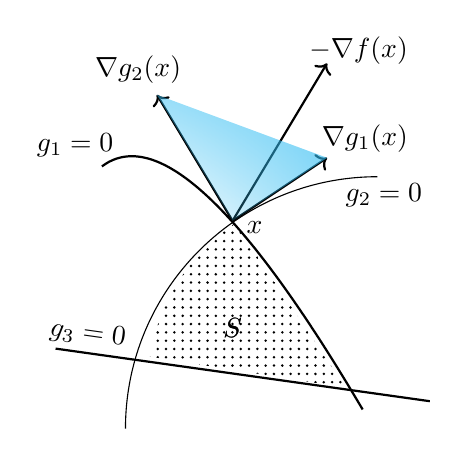
\begin{tikzpicture}[scale=0.8]
\begin{scope}[shift={(-1.8,1)}]
\draw[scale=1.5,domain=-0.2:1.8, smooth, variable=\x, black,thick,rotate=15] plot ({\x}, -{\x*\x});
\end{scope}
\begin{scope}[shift={(-5.7,-3.3)}]
\draw (4cm,0cm) arc (180:90:4cm);
\end{scope}
\draw[->,thick] (0,0)--(1.5,1);\node[black] at (2.1,1.3) {${\nabla}g_{1}(x)$};
\draw[->,thick] (0,0)--(-1.2,2);\node[black] at (-1.5,2.4) {${\nabla}g_{2}(x)$};
\draw[->,thick] (0,0)--(1.5,2.5);\node[black] at (2,2.7) {$-{\nabla}f(x)$};
\path[path fading=west,fill=cyan!80!,opacity=0.5] (0,0)-- (1.5,1) --(-1.2,2) --cycle;
\path[path fading=south,fill=cyan!80!,opacity=0.5] (0,0)-- (1.5,1) --(-1.2,2) --cycle;
\draw[-,thick,rotate=-8] (-2.5,-2.4)--(3.5,-2.4);\node[black,rotate=-8] at (-2.3,-1.8) {$g_{3} = 0$};
\node[black] at (0.35,-0.1) {$x$};\node[black] at (-2.5,1.2) {$g_{1} = 0$};\node[black] at (2.4,0.4) {$g_{2} = 0$};
\node[black] at (0,-1.7) {$S$};

\begin{scope}[shift={(1.8,-2.65)}]
\fill[pattern=dots,rotate=124] (0,0) -- (3.15cm,0cm) arc (0:47:3.15cm) -- cycle;
\end{scope}
\node[black] at (0,-1.7) {$S$};
\end{tikzpicture}
\end{center}
\end{figure}

\end{document}